\chapter{Graph Layout Algorithms}
\label{chap:graph_layout_algorithms}

Graph layout algorithms (or \glspl{GLA} for short) are a class of algorithms used for computing positions
of nodes so that they make a nice-looking or helpful diagram.
These algorithms accept graph-representing data as input and produce positions of individual nodes as output.

In this work, we are going to assume that GLAs produce 2-dimensional layouts,
but it is worth mentioning that the number of dimensions can be arbitrarily high.

There are many types of GLA, each with its strengths and weaknesses.
Let us look at some of the common ones.

\section{Circular Layout}

Circular layout (Figure \ref{obr:graph_layout_circular}) algorithms arrange nodes in a circle, often emphasizing the structure of the graph by placing nodes
with similar properties close together.
In a circular layout, nodes can be distributed evenly along the circumference of the circle,
or their placement can be weighted by specific properties (e.g., node degree or importance).

\begin{figure}[h]\centering
    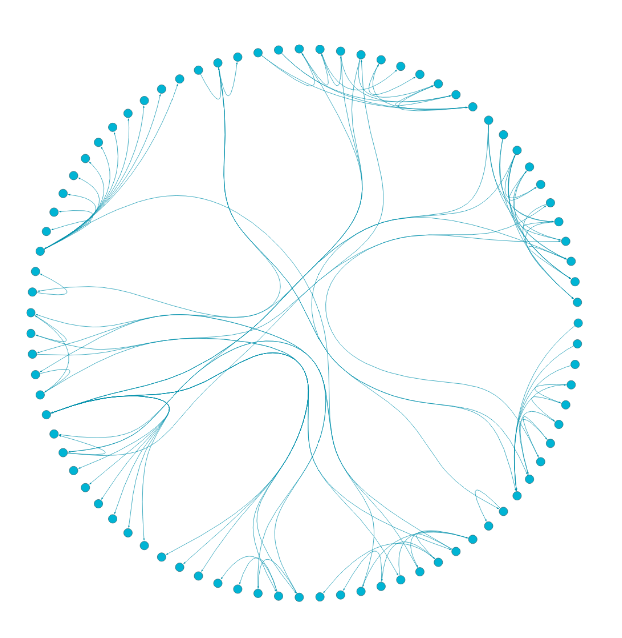
\includegraphics[width=100mm, keepaspectratio]{img/graph_layout_cicrular.png}
    \caption{Circular layout\cite{graph_layout_demos}}
    \label{obr:graph_layout_circular}
\end{figure}

\section{Hierarchical Layout}

Hierarchical layout (Figure \ref{obr:graph_layout_hierarchical})algorithms are designed to emphasize directional relationships, such as those found in flowcharts,
dependency graphs, or organizational charts. These algorithms arrange nodes in layers or levels, with edges generally
flowing in a single direction (e.g., top to bottom or left to right).

This layout can be applied to general graphs but is most effective for directed acyclic graphs (DAGs) or undirected trees.
Note that the structure in Figure \ref{obr:graph_layout_radial} is not a tree but a general graph.

\begin{figure}[h]\centering
    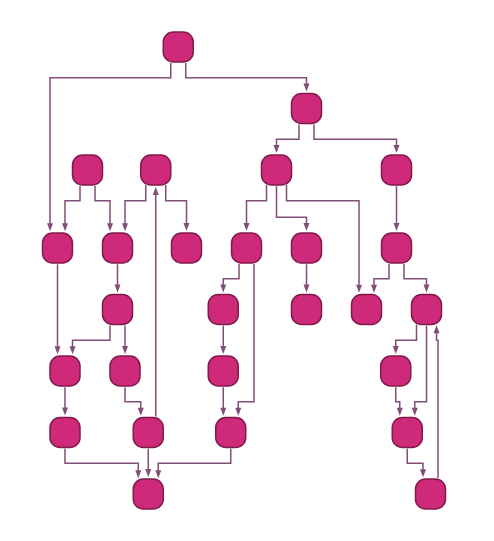
\includegraphics[width=100mm, keepaspectratio]{img/graph_layout_hiearchichal.png}
    \caption{Hierarchical layout\cite{graph_layout_demos}}
    \label{obr:graph_layout_hierarchical}
\end{figure}

\section{Radial Layout}

Radial layout (Figure \ref{obr:graph_layout_radial}) is a type of hierarchical layout where nodes are arranged in concentric circles around a central node (root).
Its immediate neighbors are arranged in the first circle. Subsequent layers represent nodes further away.
Radial layout can help highlight relationships between the central node and its surroundings.

Figure \ref{obr:graph_layout_radial} shows a tree.
In the context of social networks, many of the contemporary social networks are composed of trees:
\begin{itemize}
    \item \textbf{Reddit} - The root represents a post, and the rest are its comments
    \item \textbf{Twitter} - The root is a standalone tweet, and the rest form a series of replies
    \item \textbf{Youtube} - The root is a video, and the rest are its comments
\end{itemize}

As such, if one visualized the content of these social networks, it might look like a set of radial layouts.
We are highlighting this fact because Aphantasia's content structure is not a \gls{tree} but a \gls{DAG}
which might have interesting consequences for navigation, user experience, and usage.

\begin{figure}[h]\centering
    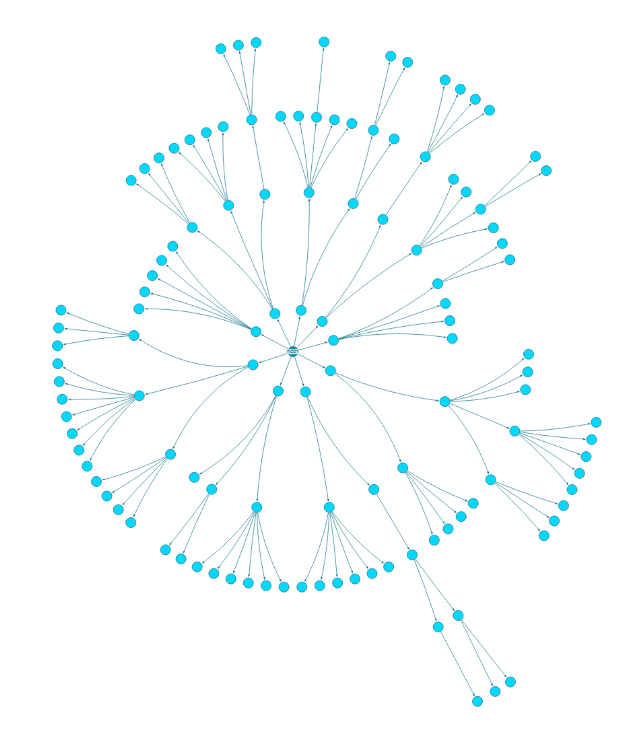
\includegraphics[width=100mm, keepaspectratio]{img/graph_layout_radial.png}
    \caption{Radial layout\cite{graph_layout_demos}}
    \label{obr:graph_layout_radial}
\end{figure}

\section{Force-Directed Layout}
\label{sec:force_directed_layout}

This type of layout is going to be the focus of this work.
All of the layouts we will present in later chapters were produced by force-directed layout (FDL) algorithms.

The main idea behind FDL algorithms is very intuitive:
Nodes are attracted to each other when connected by an edge and repelled otherwise.
Elegant in concept and easy to implement, this approach is endlessly customizable.

One particularly useful feature is that FDL algorithms are incremental and update the layout continuously.
This can be utilized to produce visually pleasing animations of the data and allows for user interaction
(e.g., dragging nodes around or changing parameters).
The dragging feature can also be used to aid the algorithm in achieving a more desired layout during its run.

Thanks to this aspect, a developer implementing an FDL algorithm has the ability to adjust the strength of the forces, add new ones,
or implement entirely new behaviors and parameters to fit specific use cases 
- all by watching the animation run, interacting with it, and inferring what behavior needs to be changed or added.

These positives are, however, balanced by two drawbacks:
\begin{itemize}
    \item \textbf{high time complexity}

 The basic version of FDL has a time complexity of $O(n^2)$ per step, where $n$ is the number of nodes in the graph.
 For stabilization, usually $n$ steps are considered sufficient,
 and thus, the time complexity for producing a stabilized graph is often computed as $O(n^3)$.

    \item \textbf{sensitive parameterization}
    
 As for parameterization, the algorithm is highly dependent on the parameters set by the user (or developer),
 some of which can be very sensitive and radically change the resulting layout with only a small change in value.
 This can be a challenge for users unfamiliar with the algorithm or the data they are working with.
 Achieving a specific look or quality for the final graph render often requires a significant amount of time spent tweaking the parameters.

 This fact also means that it is difficult to create a "one size fits all" FDL algorithm
 - the parameters that work well for one dataset might not work well for another.
\end{itemize}